\section{Why the empirical forecast wins at long horizons (exploratory)}
\label{sec:explanation}

We did not measure schedule irregularity in Berka directly, and every
analysis in this section was specified after the held-out results were
known. The comparisons below narrow the explanation down; they do not
establish one. We tested four candidate explanations, each specified in
writing before running (\texttt{paper/REVISION.md}):
\begin{itemize}
\item calendar alignment;
\item the cost of projecting the schedule;
\item sparse event counts;
\item history length;
\end{itemize}
plus an independent simulation. Every new method uses the same \R{c/lookback}-day
lookback, the same origins and the same information as B-EQ.
\begin{itemize}
\item \textbf{B-EQc} restricts B-EQ's past windows to those starting
  within \R{c/cal-half} days of the origin's day of the month.
\item \textbf{B-SR} uses B-EQ's past windows, but replaces each window's
  scheduled flows with the schedule's projection. Its samples are
  $B_t + \Delta B_{\text{hist}} - S_{\text{hist}} + S_t$: $\Delta B_{\text{hist}}$
  is a past $h$-day change (B-EQ's sample), $S_{\text{hist}}$ the realized
  flows in that window of the pay and bill streams detected at the origin
  (a retrospective decomposition, not a projection made at the past date),
  and $S_t$ the schedule's projection over the next $h$ days.
\item \textbf{CP-noKF} is V2's compound-Poisson spending model with the
  filter removed. Its paths start at today's booked balance and add the
  schedule's flows and simulated discretionary events.
\end{itemize}
All were developed on the development split (\R{xd/s3/V2-vs-B-EQ/30/forecasts}
origins per horizon) and then run once on held-out accounts in a logged
run (\R{xh/s3/V2-vs-B-EQ/30/forecasts} origins). Table~\ref{tab:explain}
gives both.

\begin{table}[t]
\centering\scriptsize\setlength{\tabcolsep}{4pt}
\begin{tabular}{l ll ll}
\toprule
 & \multicolumn{2}{c}{Development} & \multicolumn{2}{c}{Held-out}\\
\cmidrule(lr){2-3}\cmidrule(lr){4-5}
Comparison (skill of the first) & \hB\ d & \hC\ d & \hB\ d & \hC\ d\\
\midrule
B-EQc vs B-EQ & \pq{xd/s3/B-EQc-vs-B-EQ}{30} & \pq{xd/s3/B-EQc-vs-B-EQ}{90} & \pq{xh/s3/B-EQc-vs-B-EQ}{30} & \pq{xh/s3/B-EQc-vs-B-EQ}{90}\\
B-SR vs B-EQ & \pq{xd/s3/B-SR-vs-B-EQ}{30} & \pq{xd/s3/B-SR-vs-B-EQ}{90} & \pq{xh/s3/B-SR-vs-B-EQ}{30} & \pq{xh/s3/B-SR-vs-B-EQ}{90}\\
V2 vs B-EQ & \pq{xd/s3/V2-vs-B-EQ}{30} & \pq{xd/s3/V2-vs-B-EQ}{90} & \pq{xh/s3/V2-vs-B-EQ}{30} & \pq{xh/s3/V2-vs-B-EQ}{90}\\
CP-noKF vs B-EQ & \pq{xd/s3/cp-nokf-vs-b-eq}{30} & \pq{xd/s3/cp-nokf-vs-b-eq}{90} & \pq{xh/s3/cp-nokf-vs-b-eq}{30} & \pq{xh/s3/cp-nokf-vs-b-eq}{90}\\
B-EQ vs B-SA+ & \pq{xd/s3/B-EQ-vs-B-SA+}{30} & \pq{xd/s3/B-EQ-vs-B-SA+}{90} & \pq{xh/s3/B-EQ-vs-B-SA+}{30} & \pq{xh/s3/B-EQ-vs-B-SA+}{90}\\
\addlinespace
B-SR vs V2 & \pq{xd/s3/B-SR-vs-V2}{30} & \pq{xd/s3/B-SR-vs-V2}{90} & \pq{xh/s3/B-SR-vs-V2}{30} & \pq{xh/s3/B-SR-vs-V2}{90}\\
CP-noKF vs V2 & \pq{xd/s3/cp-nokf-vs-v2}{30} & \pq{xd/s3/cp-nokf-vs-v2}{90} & \pq{xh/s3/cp-nokf-vs-v2}{30} & \pq{xh/s3/cp-nokf-vs-v2}{90}\\
\bottomrule
\end{tabular}
\caption{The explanation's comparisons (exploratory): pooled CRPS skill of
the first method against the second, with the account mean in brackets
(negative: the first has higher CRPS). Same origins for all methods within
a split. Development: \R{xd/s3/V2-vs-B-EQ/30/forecasts} origins in
\R{xd/s3/V2-vs-B-EQ/30/accounts} accounts per horizon. Held-out:
\R{xh/s3/V2-vs-B-EQ/30/forecasts} in \R{xh/s3/V2-vs-B-EQ/30/accounts}.
Intervals are in the result files (\texttt{paper/results/exploratory*}).}
\label{tab:explain}
\end{table}

\paragraph{Replacing past scheduled flows with the projection.} Four
methods project the detected pay-and-bill schedule: V2, CP-noKF, B-SR and
B-SA+. All four have higher CRPS than B-EQ at \hB\ and \hC\ days, on both
splits, B-SA+ by the most (Table~\ref{tab:explain}). B-SR is the closest
contrast: on the same windows, it differs from B-EQ only by the
replacement $S_t - S_{\text{hist}}$. It loses on held-out accounts with
pooled skill \R{xh/s3/B-SR-vs-B-EQ/30/skill_pooled} and
\R{xh/s3/B-SR-vs-B-EQ/90/skill_pooled} (account mean
\R{xh/s3/B-SR-vs-B-EQ/30/skill_mean} and
\R{xh/s3/B-SR-vs-B-EQ/90/skill_mean}). Its \lC\% intervals are about as
narrow as B-EQ's (median \R{xh/s3/stats/B-SR/90/median_width90} against
\R{xh/s3/stats/B-EQ/90/median_width90} CZK at \hC\ days), so the loss is
not a matter of width.

\begin{table}[t]
\centering\scriptsize\setlength{\tabcolsep}{3.5pt}
\begin{tabular}{l lll}
\toprule
Comparison (skill of the first; development) & \hA\ d & \hB\ d & \hC\ d\\
\midrule
B-SR vs B-EQ (schedule replacement) & \pq{xd/s14/f1-vs-f0}{7} & \pq{xd/s14/f1-vs-f0}{30} & \pq{xd/s14/f1-vs-f0}{90}\\
Oracle vs B-EQ (realized future scheduled flows) & \pq{xd/s14/o-vs-f0}{7} & \pq{xd/s14/o-vs-f0}{30} & \pq{xd/s14/o-vs-f0}{90}\\
Shuffled B-EQ vs B-EQ (pairing broken) & \pq{xd/s14/eq-shuf-vs-f0}{7} & \pq{xd/s14/eq-shuf-vs-f0}{30} & \pq{xd/s14/eq-shuf-vs-f0}{90}\\
Matched B-SR vs B-SR (pairing restored) & \pq{xd/s14/sr-match-vs-f1}{7} & \pq{xd/s14/sr-match-vs-f1}{30} & \pq{xd/s14/sr-match-vs-f1}{90}\\
\addlinespace
B-SR vs B-EQ, predictable tertile & -- & \pq{xd/s11-predictable/f1-vs-f0}{30} & \pq{xd/s11-predictable/f1-vs-f0}{90}\\
B-SR vs B-EQ, middle tertile & -- & \pq{xd/s11-middle/f1-vs-f0}{30} & \pq{xd/s11-middle/f1-vs-f0}{90}\\
B-SR vs B-EQ, unpredictable tertile & -- & \pq{xd/s11-unpredictable/f1-vs-f0}{30} & \pq{xd/s11-unpredictable/f1-vs-f0}{90}\\
\bottomrule
\end{tabular}
\caption{What explains B-SR's loss (exploratory, development accounts,
\R{xd/s14/f1-vs-f0/30/forecasts} origins in \R{xd/s14/f1-vs-f0/30/accounts}
accounts per horizon; tertiles of \R{xd/s11-predictable/f1-vs-f0/30/forecasts}
origins each): pooled CRPS skill of the first forecast against the second,
account mean in brackets. Intervals are in
\texttt{paper/results/exploratory/s11-schedule/} and \texttt{s14-dependence/}.}
\label{tab:mechanism}
\end{table}

\paragraph{Projection error is not sufficient.} If B-SR lost only because
the projection $S_t$ misjudges the coming flows, replacing $S_t$ with the
flows the same streams actually produced over the horizon (an oracle,
using the future) should remove the loss. On development accounts it does
at short horizons but not at long ones: at \hC\ days the oracle still loses
to B-EQ (Table~\ref{tab:mechanism}).

\paragraph{Within-window dependence: real, but small.} Our leading
hypothesis was that B-EQ wins because each past window keeps its pay and
the spending that went with it together, while schedule-based forecasts
recombine the two. Breaking that pairing within B-EQ, by recombining each
window's scheduled flows with another window's residual, does make it
worse at \hB\ and \hC\ days under both aggregations, but only slightly
(account-mean skill \R{xd/s14/eq-shuf-vs-f0/30/skill_mean@3} and
\R{xd/s14/eq-shuf-vs-f0/90/skill_mean@3}), a small fraction of B-SR's
loss. Restoring the pairing within
B-SR, by drawing residuals only from windows whose scheduled flow resembles
the projection, makes B-SR worse, not better, though it also leaves it
fewer windows. Within-window dependence therefore explains at most a small
part of the long-horizon loss; the rest is unexplained.

\paragraph{A confirmatory forward-period test.} We fixed four predictions
from the development results above in a written specification
(\texttt{paper/REVISION.md}, S15, committed before the run), and tested them
once, in a logged run, on held-out origins dated on or after 1997-07-01
(\R{cf/pred/p2/90/origins} per horizon in \R{cf/pred/p2/90/accounts}
accounts). The primary estimand is the account mean; a prediction is
confirmed if its 95\% interval lies wholly on the predicted side. All four
were confirmed (Table~\ref{tab:s15}), and the pooled skill agrees in sign
throughout.

\begin{table}[t]
\centering\scriptsize\setlength{\tabcolsep}{3pt}
\begin{tabular}{l l l l l}
\toprule
Prediction & $h$ & Account mean [95\%] & Pooled & Verdict\\
\midrule
P2: oracle vs B-EQ, $<0$ & \hC & \R{cf/pred/p2/90/skill_mean} [\R{cf/pred/p2/90/skill_mean_lo}, \R{cf/pred/p2/90/skill_mean_hi}] & \R{cf/pred/p2/90/skill_pooled} & \R{cf/pred/p2/90/verdict}\\
P3: shuffled B-EQ vs B-EQ, $<0$ & \hB & \R{cf/pred/p3/30/skill_mean@3} [\R{cf/pred/p3/30/skill_mean_lo@3}, \R{cf/pred/p3/30/skill_mean_hi@3}] & \R{cf/pred/p3/30/skill_pooled@3} & \R{cf/pred/p3/30/verdict}\\
 & \hC & \R{cf/pred/p3/90/skill_mean@3} [\R{cf/pred/p3/90/skill_mean_lo@3}, \R{cf/pred/p3/90/skill_mean_hi@3}] & \R{cf/pred/p3/90/skill_pooled@3} & \R{cf/pred/p3/90/verdict}\\
P3b: $s_{\text{shuf}} - s_{\text{SR}}/4 > 0$ & \hC & \R{cf/pred/p3b/90/skill_mean@3} [\R{cf/pred/p3b/90/skill_mean_lo@3}, \R{cf/pred/p3b/90/skill_mean_hi@3}] & \R{cf/pred/p3b/90/skill_pooled@3} & \R{cf/pred/p3b/90/verdict}\\
P1 (secondary): $s_{\text{SR}}^{\text{pred}} - s_{\text{SR}}^{\text{unpred}} > 0$ & \hB & \R{cf/pred/p1-secondary/30/skill_mean} [\R{cf/pred/p1-secondary/30/skill_mean_lo}, \R{cf/pred/p1-secondary/30/skill_mean_hi}] & \R{cf/pred/p1-secondary/30/skill_pooled} & \R{cf/pred/p1-secondary/30/verdict}\\
 & \hC & \R{cf/pred/p1-secondary/90/skill_mean} [\R{cf/pred/p1-secondary/90/skill_mean_lo}, \R{cf/pred/p1-secondary/90/skill_mean_hi}] & \R{cf/pred/p1-secondary/90/skill_pooled} & \R{cf/pred/p1-secondary/90/verdict}\\
\bottomrule
\end{tabular}
\caption{The forward-period confirmatory test S15 on held-out Berka
(origins on or after 1997-07-01; P1 on the \R{cf/pred/p1-secondary/30/origins}
origins in the two outer tertiles). P2 and P3: CRPS skill of the first forecast
against the second. P3b: shuffled B-EQ's loss against B-EQ is under a
quarter of B-SR's, tested as $s_{\text{shuf}} - s_{\text{SR}}/4 > 0$ with both
skills against B-EQ. P1: B-SR's skill against B-EQ is higher in the
predictable than in the unpredictable tertile, tested on the difference.
Each with
\R{c/ci-level}\% account-bootstrap intervals. On these origins B-SR's
account-mean skill against B-EQ at \hC\ days is \R{cf/f1-vs-f0/90/skill_mean}
(\texttt{paper/results/confirmatory-s15/}).}
\label{tab:s15}
\end{table}

What the test does and does not show. It confirms, on held-out accounts and
a later period, that even exact future scheduled flows do not rescue the
replacement at \hC\ days, that within-window dependence is real but small
next to the schedule-based loss, and that replacement does relatively
better where schedules were predictable. It does not identify what causes
the loss. \emph{Prior exposure:} before the specification we had seen the
frozen held-out evaluation and the exploratory held-out results of
\S\ref{sec:reversal} and this section, including held-out B-SR against
B-EQ over all origins, which include the post-cutoff ones; we had not seen
any held-out result for the oracle, for shuffled B-EQ, by predictability
tertile, or restricted to the post-cutoff period. The cutoff date was
chosen from the calendar.

\paragraph{An open hypothesis: does the adjustment widen the sampled
changes?} One possibility is that subtracting each window's realized
scheduled flows leaves residuals that are more dispersed than the raw
changes. A descriptive check on development accounts (exploratory, S16)
does not support it: the 5--95\% range of $\Delta B_{\text{hist}} -
S_{\text{hist}}$ is wider than that of $\Delta B_{\text{hist}}$ at
\R{xd/s16/90/share_origins_wider}\% of origins at \hC\ days
(\R{xd/s16/30/share_origins_wider}\% at \hB), and the median per-account
ratio of the two ranges is \R{xd/s16/90/ratio_median} (quartiles
\R{xd/s16/90/ratio_q25} and \R{xd/s16/90/ratio_q75}). Spread is therefore
not obviously the cause; how the residuals are located relative to the
coming flows remains an open question.

\paragraph{Schedule predictability: weak, aggregation-dependent effects.}
We measured, from each origin's own history, how far the schedule
detected at earlier checkpoints missed the next month's scheduled flows,
and split origins into tertiles. On the pooled score, schedule replacement
helps slightly in the most predictable tertile and hurts in the others.
Under the planned account mean it hurts in every tertile
(Table~\ref{tab:mechanism}), and the middle tertile does worst. The
relative pattern (better in the predictable tertile than in the
unpredictable one) was confirmed in the forward-period test above.

\paragraph{History length: weaker, aggregation-dependent evidence.} If
B-EQ needed a long history to represent the distribution of changes, the
gap should shrink for short histories. It does only when scores are
pooled over origins, which weights the accounts with large errors more.
Under the planned account mean, B-EQ keeps a clear long-horizon advantage
with under a year of history, on both splits:

\begin{center}\footnotesize
\begin{tabular}{lll}
\toprule
V2 vs B-EQ, pooled (account mean) & under 12 months & 24 months or more\\
\midrule
Development, \hB\ d & \pq{xd/s3-history-lt12/V2-vs-B-EQ}{30} & \pq{xd/s3-history-ge24/V2-vs-B-EQ}{30}\\
Development, \hC\ d & \pq{xd/s3-history-lt12/V2-vs-B-EQ}{90} & \pq{xd/s3-history-ge24/V2-vs-B-EQ}{90}\\
Held-out, \hB\ d & \pq{xh/s3-history-lt12/V2-vs-B-EQ}{30} & \pq{xh/s3-history-ge24/V2-vs-B-EQ}{30}\\
Held-out, \hC\ d & \pq{xh/s3-history-lt12/V2-vs-B-EQ}{90} & \pq{xh/s3-history-ge24/V2-vs-B-EQ}{90}\\
\bottomrule
\end{tabular}
\end{center}

At \hC\ days the gap is largest at 12--23 months, not at the longest
histories, under both aggregations and on both splits. Whether
B-EQ's advantage depends on the number of past windows is therefore not
settled by these data.

\paragraph{Simulation: schedule regularity, not sparsity.} We crossed four
levels of spending sparsity, from \R{xd/s4/0/0/V2-vs-B-EQ/30/mean_count} down
to \R{xd/s4/3/0/V2-vs-B-EQ/30/mean_count} purchases a day, with four levels
of schedule regularity. The regularity factors are pay-date jitter,
paycheck amount noise and bill drift. Figure~\ref{fig:grid} shows the
result:
\begin{itemize}
\item \textbf{Regular schedules:} V2 has lower CRPS than B-EQ at every
  sparsity, including the sparsest
  (\R{xd/s4/3/1/V2-vs-B-EQ/30/skill_pooled} at \hB\ days).
\item \textbf{The most irregular level:} B-EQ wins at every sparsity
  (\R{xd/s4/3/3/V2-vs-B-EQ/30/skill_pooled} in the sparsest cell).
\item \textbf{Sparsity alone} shrinks V2's lead but never reverses it.
\end{itemize}
In our generator, B-EQ's advantage at \hB\ and \hC\ days needs irregular
schedules. On Berka, the predictability tertiles give only weak support for
the same pattern. The simulation covers \hB\ and \hC\ days
only, and varies the three regularity factors together.

\begin{figure}[t]
\centering
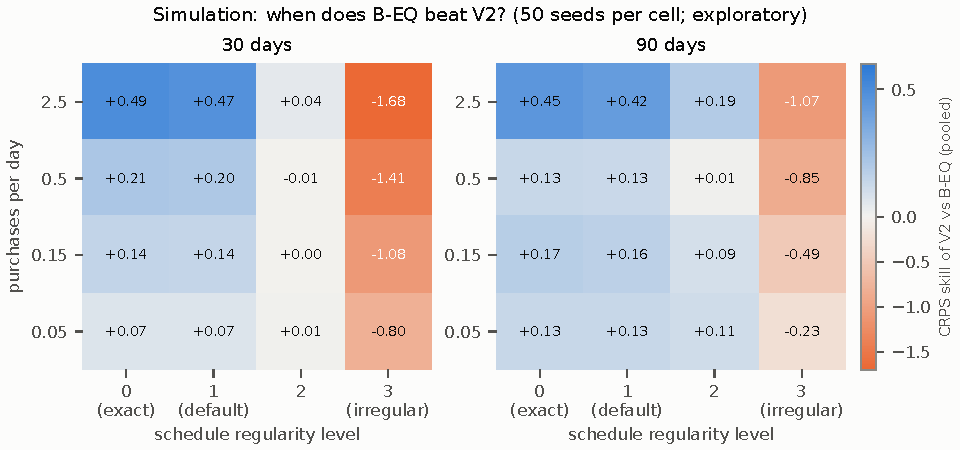
\includegraphics[width=0.85\linewidth]{figures/grid-synthetic.pdf}
\caption{Simulation (exploratory): pooled CRPS skill of V2 against B-EQ by
spending sparsity and schedule regularity, \R{xd/s4/0/0/V2-vs-B-EQ/30/accounts}
seeds and \R{xd/s4/0/0/V2-vs-B-EQ/30/forecasts} origins per cell and
horizon. Blue: V2 has lower CRPS; orange: B-EQ does. Seed-bootstrap
intervals are in \texttt{paper/results/exploratory/s4-grid/}.}
\label{fig:grid}
\end{figure}

\paragraph{Calendar alignment and sparse event counts, as tested.}
\begin{itemize}
\item \textbf{Calendar alignment.} The one rule we tested, restricting
  B-EQ's past windows to those starting within \R{c/cal-half} days of the
  origin's day of the month, makes it slightly \emph{worse} on both splits
  (Table~\ref{tab:explain}). It also leaves B-EQ fewer windows, so it does
  not rule out other forms of calendar alignment.
\item \textbf{Sparse event counts.} Modelling spending as sparse discrete
  events without the filter (CP-noKF) loses to B-EQ by about as much as V2
  does. In our generator, over the sparsity range tested
  (\R{xd/s4/0/0/V2-vs-B-EQ/30/mean_count} to
  \R{xd/s4/3/0/V2-vs-B-EQ/30/mean_count} purchases a day), sparsity alone did
  not give B-EQ the advantage. The filter itself helps a little: removing
  it (CP-noKF against V2) raises CRPS slightly on both splits.
\end{itemize}

\paragraph{Origin phase.} The size of the \hB-day gap depends on where
in the month the origins fall. On development accounts, on grids shifted
by +10 and +20 days, V2's pooled skill against B-EQ is
\R{xd/s8-offset10/V2-vs-B-EQ/30/skill_pooled} and
\R{xd/s8-offset20/V2-vs-B-EQ/30/skill_pooled} (account mean
\R{xd/s8-offset10/V2-vs-B-EQ/30/skill_mean} and
\R{xd/s8-offset20/V2-vs-B-EQ/30/skill_mean}), against
\R{xd/s3/V2-vs-B-EQ/30/skill_pooled}
(\R{xd/s3/V2-vs-B-EQ/30/skill_mean}) on the frozen grid. The sign holds on
every grid.

\paragraph{What we did not show.} None of these analyses identifies why
B-EQ wins at long horizons. Projection error and within-window dependence
each explain a part at most, the simulation uses our own generator, and
every analysis here followed the held-out results. The schedule
irregularity the simulation varies was measured on Berka only through the
predictability tertiles above, whose effects are weak.
